Am 26. Januar 2021 veröffentlichte das \ac{W3C} die \ac{WebRTC} Recommendation. Eine Recommendation des \acs{W3C} ist dabei ein offizieller Web-Standard in seiner -- bezüglich der zentralen Funktionalität -- finalen Form. \acs{WebRTC} ist eine Peer-To-Peer Web-Technologie, und wird primär für Echtzeit-Applikationen wie Audio- und Videochats verwendet.\par

Die Beliebtheit von interaktiven Mehrspieler-Brettspielen, welche durch das einfache Abrufen einer Webseite spielbar sind, steigt von Jahr zu Jahr, nicht zuletzt bedingt durch die seit März 2020 andauernde Covid-19 Pandemie. Die Auswahl an verschiedenen Spielarten fällt dabei divers aus -- von Schach bis hin zu Karten- oder Gesellschaftsspielen, wie zum Beispiel Monopoly.\par

In der Regel basieren diese Spiele auf einer Client-Server-Architektur, wobei der Server die Rolle des bestimmenden Spielleiters übernimmt. Dabei werden sämtliche Aktionen eines Spielers über den Server validiert, und mit anderen Spielern synchronisiert. Die Clients sind dabei lediglich für die Darstellung des vom Server verwalteten Spielstands zuständig.\cite{bura2012}\par

Ein weiterer, gut definierter und häufig genutzter Ansatz für die Vernetzung von Spielern ist die \acs{P2P} Architektur. Bei dieser existiert kein zentraler Server, die Nutzer (Peers) sind gleichberechtigt und tauschen Daten direkt untereinander aus. Das Spiel wird dabei entweder von einem der Peers (dem sogenannten 'Host') orchestriert, oder ist auf alle Peers verteilt. Einer der großen Vorteile der Peer-To-Peer Architektur sind dabei die geringeren Datenmengen, welche über einen zentralen Server verwaltet werden müssen. Dies führt zu Kostenersparnissen in Form von weniger Bedarf an Hardware.\par

Beide dieser Netzwerkarchitekturen finden in der Spieleentwicklung Anwendung -- jedoch ist die Nutzung von Peer-To-Peer zum Datenaustausch bei Browserbasierten Mehrspieler-Spielen begrenzt. Dies ist nicht zuletzt auf das Lebensende des Adobe Flash Players im Dezember 2020 zurückzuführen, welcher über Peer-To-Peer Fähigkeiten, ermöglicht durch das Real-Time Media Flow Protocol von Adobe, verfügte. Seitdem existiert -- mit Ausnahme von \acs{WebRTC} -- keine alternative Möglichkeit um Nutzer von Web-Applikationen, ohne die Nutzung von Plug-Ins oder Drittanbietersoftware, direkt untereinander zu vernetzen.\par

\section{WebRTC in Browserbasierten Mehrspieler-Spielen}
\acs{WebRTC} wird bereits in einigen Mehrspieler-Spielen, sowie Networking- und Spiel-Frameworks verwendet. In der Regel wird WebRTC dabei jedoch lediglich für Sprach- und Videokommunikation eingesetzt. Die Strategie- und Brettspiel Plattform \textit{Jocly} ist eine der ersten Plattformen, welche bereits seit 2013 \acs{WebRTC} nutzt, damit Spieler sich in Echtzeit über ihre Webcams beim Spielen sehen, sowie miteinander kommunizieren können\cite{jocly2013} (vgl. Abbildung 1). Ähnlich verhält es sich bei einigen weiteren Frameworks, wie zum Beispiel \textit{Tabloro}\footnote{vgl. \url{https://github.com/fyyyyy/tabloro}}.

\begin{figure}[h]
\centering
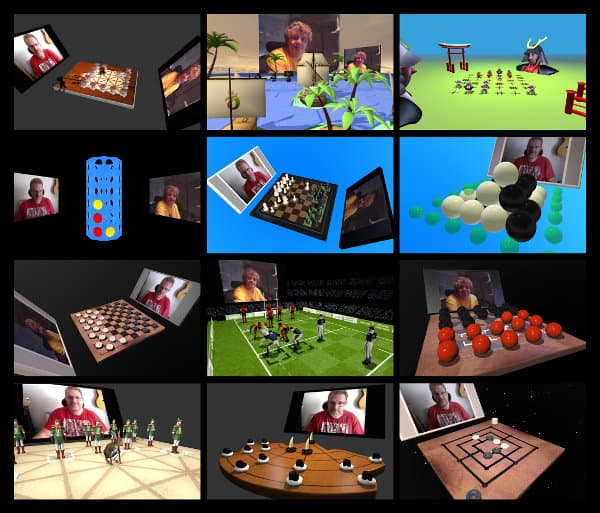
\includegraphics[width=0.75\textwidth]{bilder/jocly-games.jpg}
\caption{Screenshots einiger Jocly-Spiele.}
\end{figure}

\color{red}
Es existieren zudem einige Spiele sowie Frameworks, welche WebRTC zum Austausch von Spielrelevanten Daten nutzen. Bei diesen handelt es sich jedoch in der Regel um Prototypen und Frameworks, welche auf Echtzeit-Applikationen ausgelegt sind. Zum Beispiel die Netzwerk-Bibiliothek \textit{HumbleNet}. Bei HumbleNet handelt es sich um eine Peer-To-Peer Bibliothek zum portieren von Peer-To-Peer Spielen in Browserumgebungen\cite{humblenet}.\par
\color{black}

Weiterhin existieren eine Reihe an prototypischen Spielen, welche \acs{WebRTC} zum Austausch von Daten nutzen. Bei diesen handelt es sich überwiegend um Echtzeit-Spiele wie das 2013 von Google entwickelte \textit{Cube Slam}\footnote{vgl. \url{https://experiments.withgoogle.com/cube-slam}}, oder den von Mozilla entwickelten First-Person-Shooter \textit{Bananabread}\footnote{vgl. \url{https://hacks.mozilla.org/2013/03/webrtc-data-channels-for-great-multiplayer/}}, welche \acs{WebRTC} zum direkten Austausch von Spielrelevanten Daten zwischen Spielern nutzen.\\
TODO: Falsch - CubeSlam nutzt WebRTC auch nur für integrierten Videochat\par

Im Bereich der Rundenbasierten Brettspieleentwicklung findet WebRTC hingegen nur begrenzt Anwendung. Diese beschränkt sich primär auf die zuvor beschriebene Nutzung für Audio- und Videokommunikation.

\section{Zielsetzung}
In dieser Arbeit soll ein Brettspiel, sowie sämtliche benötigten Komponenten zum Aufbau von Peer-To-Peer Netzwerken via \acs{WebRTC}, prototypisch entworfen, implementiert und aufgesetzt werden. Ziel ist es, darauf basierend die Anwendbarkeit von \acs{WebRTC} für die Entwicklung von Brettspielen im Browser unter Nutzung von Peer-To-Peer Netzwerken zu evaluieren. Dabei soll primär auf Vor- und Nachteile einer Nutzung von Peer-To-Peer Netzwerken via \acs{WebRTC} im Vergleich zu Client-Server Modellen eingegangen werden.

\section{Aufbau der Arbeit}
Im Kapitel ‘Grundlagen’ werden zunächst \acs{WebRTC} an sich, sowie weitere verwendete Web-Technologien beschrieben, um eine Theoretische Grundlage für die spätere Implementierung zu schaffen.\par

Daraufhin wird das Design, sowie die Implementation einer \acs{WebRTC}-Infrastruktur im nächsten Kapitel beschrieben. Zudem werden die benötigten Server prototypisch in der Microsoft-Azure Cloud aufgesetzt.\par

Basierend auf der, im vorherigen Kapitel implementierten WebRTC Infrastruktur wird eine prototypische Web-Applikation erstellt, welche mehreren Spielern das Spielen des Brettspiels ‘Mensch ärgere Dich Nicht’ ermöglicht. Dieses Spiel wurde gewählt, da es mit mehr als zwei Spielern spielbar ist, und das Regelwerk des Spiels hinreichende Komplexität aufweist, um den Peer-To-Peer Ansatz auf die Probe zu stellen.\par

Daraufhin werden -- basierend auf der Implementation des Spiels und der unterliegenden Netzwerkinfrastruktur -- die Limitationen sowie Möglichkeiten, welche WebRTC im Umfeld der Spieleentwicklung im Browser eröffnet diskutiert. Diese wird primär mit Client-Server Architektur verglichen.\par

Am Ende dieser Arbeit folgt ein abschließendes Fazit, sowie ein Ausblick für weitere Arbeit in diesem Themenbereich.
